\documentclass[12pt]{article}
\usepackage[left=.5in, right=.5in, top=.5in, bottom=.5in]{geometry}
\usepackage[parfill]{parskip}
\usepackage{amsmath, amssymb, enumitem, graphicx}
\pagenumbering{gobble}
\setlength\parindent{0pt}

\begin{document}

\begin{center}
{\Large CSC413H1 - Assignment 4}
\end{center}

\textbf{1.1.2:} Given the weights $w_1,\ldots,w_n$, denote $h_0 = x$ and $h_i = \text{ReLU}(w_ih_{i-1})$ for $i\in\{1,\ldots,n\}$ such that $f(x) = h_n$. Then, \begin{align*}
    \frac{\partial h_i}{\partial h_{i-1}} &= w_i \cdot \frac{d}{dh_{i-1}} \text{ReLU}(w_ih_{i-1}) = w_i \cdot \mathbb{I}(w_ih_{i-1}>0)\\
    \frac{\partial f(x)}{\partial x} &= \prod_{i=1}^n \frac{\partial h_i}{\partial h_{i-1}} = \prod_{i=1}^n w_i \cdot \mathbb{I}(w_ih_{i-1}>0) \text{ by the chain rule}
\end{align*} for all $i$. Note that $|\frac{\partial f(x)}{\partial x}| \geq 0$ by definition and $|\frac{\partial f(x)}{\partial x}| \leq \prod_{i=1}^n |w_i|$ if all of the indicator functions evaluate to 1. The gradient does not necessarily have to vanish or explode. It vanishes when any $w_i = 0$, when $x=0$, when $x<0$ and $w_1>0$, when $x<0$ and any $w_i<0$ for $i>1$, or when $x>0$ and any $w_i<0$. It explodes when the $w_i$'s are large.

\textbf{1.2.1:} Denote $S(x) = \text{sigmoid}(x)$ and note that $S'(x) \leq \frac{1}{4}$. Since the Jacobian of $S(Wx_t)$ for all $t$ is a diagonal matrix with entries $\leq\frac{1}{4}$, its singular values are therefore also $\leq\frac{1}{4}$. In other words, $\sigma_{\text{max}}(\frac{\partial S(Wx_t)}{\partial Wx_t}) = \frac{1}{4}$. Then, by the chain rule and the hint, \begin{align*}
    \frac{\partial x_n}{\partial x_1} &= \prod_{i=1}^{n-1} \frac{\partial x_{t+1}}{\partial x_t} = \prod_{i=1}^{n-1} \frac{\partial S(Wx_t)}{\partial x_t} = \prod_{i=1}^{n-1} \frac{\partial S(Wx_t)}{\partial Wx_t} \frac{\partial Wx_t}{\partial x_t} = \prod_{i=1}^{n-1} \frac{\partial S(Wx_t)}{\partial Wx_t}W\\
    \sigma_{\text{max}}(\frac{\partial x_n}{\partial x_1}) &\leq \prod_{i=1}^{n-1} \sigma_{\text{max}} (\frac{\partial x_{t+1}}{\partial x_t}) \leq \prod_{i=1}^{n-1} \sigma_{\text{max}}(\frac{\partial S(Wx_t)}{\partial Wx_t}) \sigma_{\text{max}}(W) = \prod_{i=1}^{n-1} \frac{1}{4} \cdot \frac{1}{4} = (\frac{1}{16})^{n-1}
\end{align*} and furthermore singular values are non-negative by convention, so $0\leq \sigma_{\text{max}}(\frac{\partial x_n}{\partial x_1})\leq (\frac{1}{16})^{n-1}$.

\textbf{1.3.1:} Assume that each vector-vector product has $\mathcal{O}(1)$ time. Substituting in the kernel function yields \begin{align*}
    \alpha_i = \frac{\sum_{j=1}^n k(Q_i,K_j)V_j}{\sum_{j=1}^n k(Q_i,K_j)} = \frac{\sum_{j=1}^n \phi(Q_i)^T \phi(K_j)V_j}{\sum_{j=1}^n \phi(Q_i)^T \phi(K_j)} = \frac{\phi(Q_i)^T \sum_{j=1}^n \phi(K_j)V_j}{\phi(Q_i)^T \sum_{j=1}^n \phi(K_j)}
\end{align*} and notice that $\sum_{j=1}^n \phi(K_j)V_j$ and $\sum_{j=1}^n \phi(K_j)$ can be precomputed and stored in $\mathcal{O}(n)$ time. Thus, computing the $\alpha_i$'s for $i\in\{1,\ldots,n\}$ takes $\mathcal{O}(n)$ time in total.

\textbf{1.3.2:} Denote the low-rank SVD of $P$ as $\begin{bmatrix} u_1 & \ldots & u_k \end{bmatrix} \text{diag}(\sigma_1, \ldots, \sigma_k) \begin{bmatrix} v_1 & \cdots & v_k \end{bmatrix}^T$ for $n$-dimensional vectors $u_i, v_i \in \mathbb{R}^n$ and singular values $\sigma_i \in \mathbb{R}$. Then, the self-attention involves computing the following: \begin{itemize}
    \item $M_1 := \begin{bmatrix} v_1 & \cdots & v_k \end{bmatrix}^T V$, which is multiplying a $k\times n$ matrix with a $n\times d$ matrix and takes $\mathcal{O}(nkd)$ time;
    \item $M_2 := \text{diag}(\sigma_1, \ldots, \sigma_k) M_1$, which is multiplying each singular value with the corresponding $d$-dimensional row and takes $\mathcal{O}(kd)$ time;
    \item $\begin{bmatrix} u_1 & \ldots & u_k \end{bmatrix}^T M_2$, which is multiplying a $n\times k$ matrix with a $k\times d$ matrix and takes $\mathcal{O}(nkd)$ time.
\end{itemize} Thus, the total time complexity is $\mathcal{O}(nkd)$.

\textbf{1.4.1:} Assume that $x$ is indexed from 0 to $n-1$ inclusive so that the matrix of $\alpha$'s is \begin{align*} \begin{bmatrix}
    \alpha_{1,0} & \ldots & \alpha_{1,n-1}\\
    \vdots & \ddots & \vdots\\
    \alpha_{n,0} & \ldots & \alpha_{n,n-1}\\
\end{bmatrix} \end{align*} and $p = \{p_{-n+2},\ldots,p_n\}$. Set $p_1 = \ln 2$, $p_{-1} = 0$, $p_k = -\infty$ for all other $k$'s, $W_Q = W_K = 0$, and $W_V = \sum_{k=-n+2}^n \exp(p_k) = \exp(p_1) + \exp(p_{-1}) = 3$. This is equivalent to the convolution since for $i \in \{1,\ldots,n-2\}$, \begin{align*}
     \text{softmax}(\alpha(W_Qx,W_Kx,p))_i W_Vx &= \text{softmax} (\begin{bmatrix} \ldots & \alpha_{i,i-1} & \alpha_{i,i} & \alpha_{i,i+1} & \ldots \end{bmatrix}) W_Vx \\
     &= \text{softmax} (\begin{bmatrix} \ldots & p_1 & p_0 & p_{-1} & \ldots \end{bmatrix}) W_Vx\\
     &= \begin{bmatrix} \ldots & \frac{2}{3} & 0 & \frac{1}{3} & \ldots \end{bmatrix} 3x\\
    &= 2x_{i-1} + x_{i+1} = \text{Conv1D}(x;w)_i
\end{align*} and for $i = n-1$, $\text{softmax}(\alpha(W_Qx,W_Kx,p))_{n-1} W_Vx = \begin{bmatrix} \ldots & \frac{2}{3} & 0 \end{bmatrix} W_Vx = 2x_{n-2} = \text{Conv1D}(x;w)_{n-1}$ where $x_n = 0$ due to zero-padding. Note that any values of $p_1$ and $p_{-1}$ such that $p_1 = p_{-1} + \ln 2$ work.

\textbf{1.4.2:} Assume that $x$ is indexed from 1 to $n$ inclusive so that the matrix of $\alpha$'s is \begin{align*} \begin{bmatrix}
    \alpha_{1,1} & \ldots & \alpha_{1,1}\\
    \vdots & \ddots & \vdots\\
    \alpha_{n,1} & \ldots & \alpha_{n,n}\\
\end{bmatrix} \end{align*} and $p = \{p_{-n+1},\ldots,p_{n-1}\}$. Set $p_{k'} = 0$ for $k' \in \{-k,\ldots,k\}$ and $-\infty$ otherwise, $W_V = 1$, and $W_Q = W_K = c$ for some large constant $c$, such as $100$. Also, note that $\sqrt{d_k} = 1$. This approximates max pooling since for $i \in \{k+1,\ldots,n-k\}$, \begin{align*}
    \text{softmax}(\alpha(W_Qx,W_Kx,p))_i W_Vx &= \text{softmax} (\begin{bmatrix} \ldots & \alpha_{i,i-k} & \ldots & \alpha_{i,i+k} & \ldots \end{bmatrix}) W_Vx \\
    &= \text{softmax} (\begin{bmatrix} \ldots & c^2 x_i x_{i-k} + p_k & \ldots & c^2 x_i x_{i+k} + p_{-k} & \ldots \end{bmatrix}) W_Vx\\
    &= \begin{bmatrix} \ldots & s_i \exp(c^2 x_i x_{i-k}) & \ldots & s_i \exp(c^2 x_i x_{i+k}) & \ldots \end{bmatrix} x\\
    &= s_i \exp(c^2 x_i x_{i-k})x_{i-k} + \ldots + s_i \exp(c^2 x_i x_{i+k})x_{i+k}\\
    &\approx \max(x_{i-k},\ldots,x_{i+k}) = \text{MaxPool}(x)_i
\end{align*} where $s_i = \sum_{j=i-k}^{i+k} \exp(x_i x_j)$ and the last line holds since:
\begin{itemize}
    \item if there is one maximum $x_j \in \{x_{i-k},\ldots,x_{i+k}\}$, $s_i\exp(c^2 x_i x_j)x_j \approx x_j$;
    \item if there are multiple maximums $x_j \in \{x_{i-k},\ldots,x_{i+k}\}$, $\sum_{x_j} s_i\exp(c^2 x_i x_j)x_j \approx x_j$.
\end{itemize}

\textbf{2.1.1:} Pick $c = 72$ and let $n \in \mathbb{N}$ and $\delta > 0$. If $\delta \geq 1$, by the Cauchy-Schwarz inequality, there are infinitely many $u_i \in \mathbb{R}^n$ such that $||u_i||_2 = 1$ and $|u_i^T u_j| \leq ||u_i||_2^2 ||u_j||_2^2 = 1 \leq \delta$ where $i\neq j$, in which case the claim is satisfied.

If $\delta < 1$, define $\epsilon = \delta/3$ and $d = \lfloor \exp(n\delta^2/c) \rfloor - 1$. Using $X \subset \mathbb{R}^d$ from the hint and the JL lemma, we have that $8\ln(d+1)/\epsilon^2 = c\ln(\lfloor \exp(\frac{n\delta^2}{c}) \rfloor)/\delta^2 \leq n$, implying there exists a $n\times d$ matrix $M$ satisfying the JL inequality. Then, take this $M$ and notice that for each $(0,e_i)$ pair, \begin{align}
        1-\epsilon = (1-\epsilon)||e_i||_2^2 \leq ||Me_i||_2^2 \leq (1+\epsilon)||e_i||_2^2 = 1+\epsilon
\end{align} and for each $(e_i,e_j)$ pair where $i\neq j$, we have $||e_i-e_j||_2^2 = 2$, so \begin{align*}
    &2(1-\epsilon) = (1-\epsilon)||e_i-e_j||_2^2 \leq ||Me_i-Me_j||_2^2 \leq (1+\epsilon)||e_i-e_j||_2^2 = 2(1+\epsilon)\\
    \implies &2(1-\epsilon) \leq ||Me_i||_2^2 + ||Me_j||_2^2 - 2(Me_i)^T(Me_j) \leq 2(1+\epsilon)\\
    \implies &\frac{||Me_i||_2^2}{2} + \frac{||Me_j||_2^2}{2} - (1+\epsilon) \leq (Me_i)^T(Me_j) \leq \frac{||Me_i||_2^2}{2} + \frac{||Me_j||_2^2}{2} - (1-\epsilon)\\
    \implies &|(Me_i)^T(Me_j)| \leq 2\epsilon\\
    \implies &\left| \frac{(Me_i)^T}{||Me_i||_2^2} \frac{(Me_j)}{||Me_j||_2^2} \right| \leq \left|\frac{(Me_i)^T}{\sqrt{1-\epsilon}} \frac{(Me_j)}{\sqrt{1-\epsilon}} \right| \leq \frac{2\epsilon}{1-\epsilon} = \frac{2\delta}{3-\delta} < \frac{2\delta}{2} = \delta
\end{align*} where the second line follows from the hint, the fourth line follows from (1), and the last line follows from (1), the fourth line, and the fact that $\delta < 1 \implies 3 - \delta > 2$. Finally, define $U = \{Me_i/||Me_i||_2^2\}_{i=1}^d$ such that $|U| = d \in \Omega(\exp(n\delta^2/c))$; $\forall u\in U$, $||u||_2 = 1$; and $\forall u_i,u_j\in U$ where $i\neq j$, $|u_i^Tu_j| \leq \delta$ by the result above.

\textbf{3.1:} See the attached code.

\textbf{3.2:} See the attached code.

\textbf{3.3:} The output is shown below:
\begin{center}
    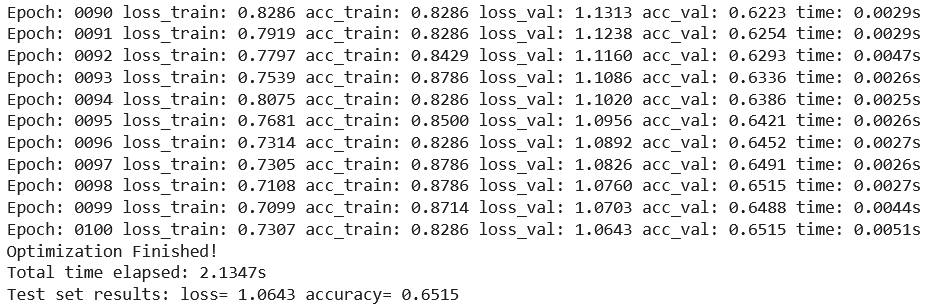
\includegraphics[width=0.75\textwidth]{3.3.png}
\end{center}

\textbf{3.4:} See the attached code.

\textbf{3.5:} The output is shown below:
\begin{center}
    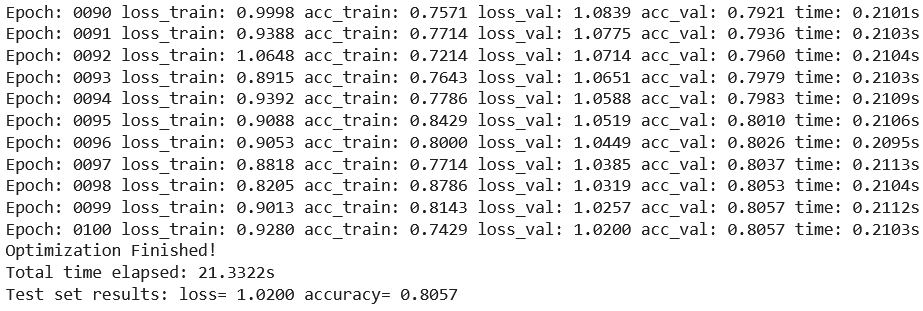
\includegraphics[width=0.75\textwidth]{3.5.png}
\end{center}

\textbf{3.6:} The GAT performed better than the vanilla GCN with a lower test loss (1.0200 vs. 1.0643) and a significantly higher test accuracy (0.8057 vs. 0.6515). This is likely because the attention layer allows the GAT to learn more features from the nodes, which improves its ability to generalize to different graphs.

\textbf{4.1:} See the attached code.

\textbf{4.2:} The outputs with skip connections disabled are shown below:
\begin{center}
    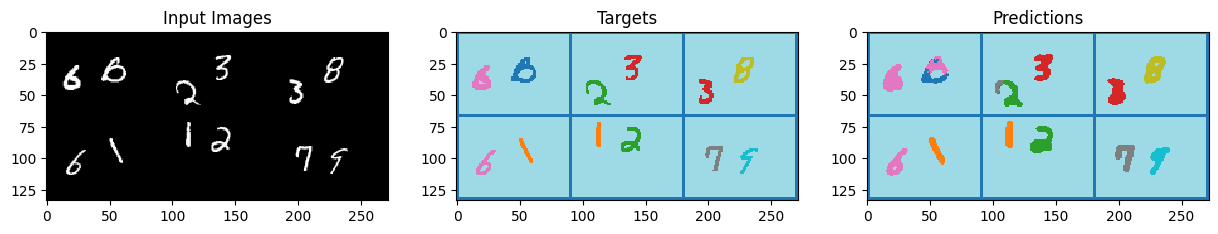
\includegraphics[width=0.75\textwidth]{4.2-1.png}
    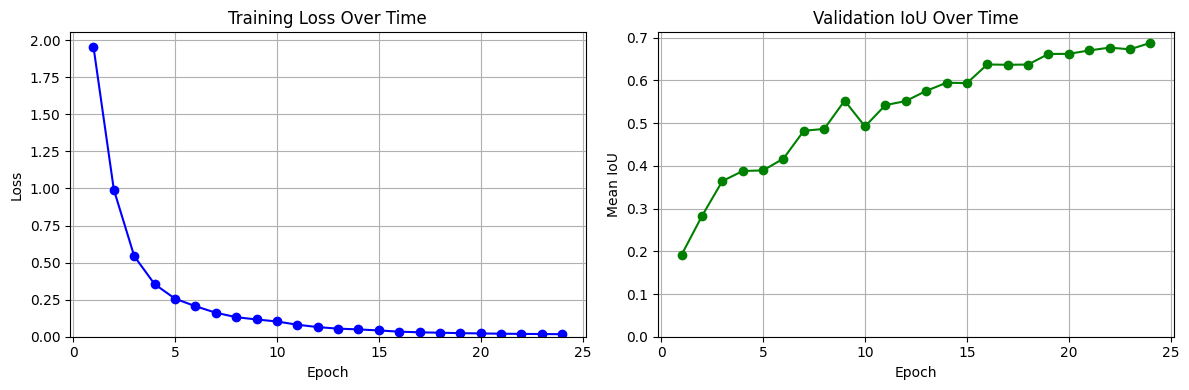
\includegraphics[width=0.75\textwidth]{4.2-2.png}
\end{center}

The outputs with skip connections enabled are shown below:
\begin{center}
    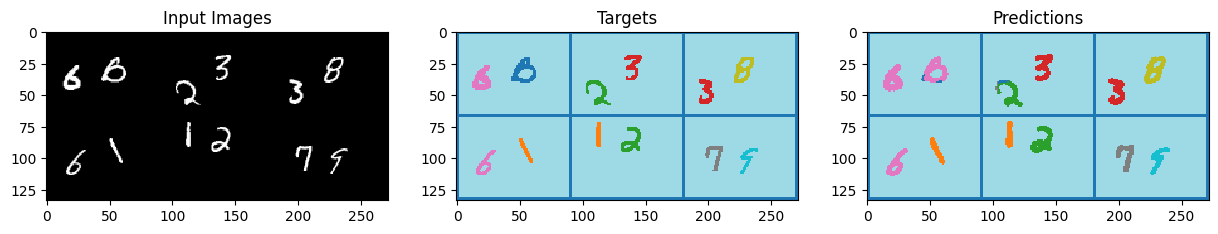
\includegraphics[width=0.75\textwidth]{4.2-3.png}
    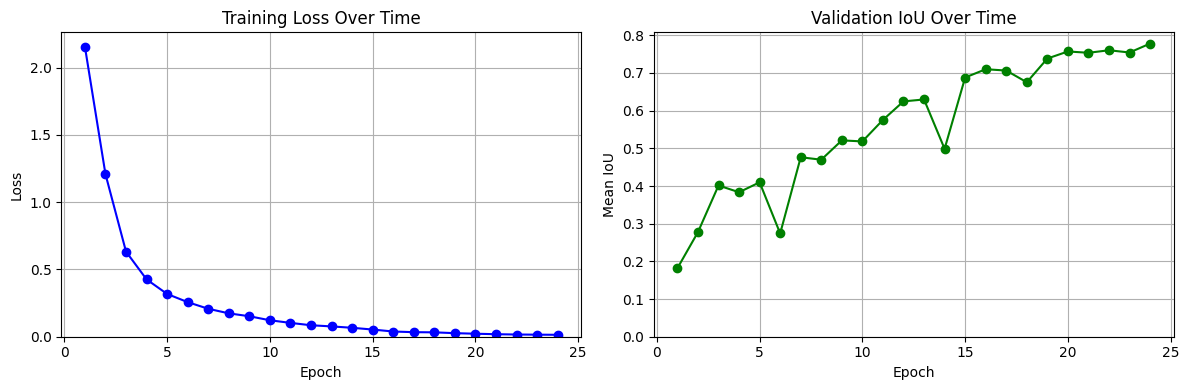
\includegraphics[width=0.75\textwidth]{4.2-4.png}
\end{center} The U-Net performed better when skip connections were enabled: it had a higher mean validation IoU (around 0.78 vs. around 0.68) and its predicted segmentations resembled the targets more. This improvement is likely because skip connections help prevent a loss of information and instability in gradients.

\end{document}